\FloatBarrier
\section{Method list}\label{app:methods}
All methods are our own implementations (\texttt{code/src/methods*.py}); the released \texttt{benchpred} package is not used. Selection and all fitting use source models only. Roles: P = proposed, B = baseline (faithful re-implementation of the textbook or published form), V = simplified variant under its own name, A = ablation, R = reference row.
\begin{center}\scriptsize
\begin{tabular}{@{}l>{\raggedright\arraybackslash}p{4.4cm}l p{5.3cm}@{}}
\toprule
Label (paper) & code name & role & description \\
\midrule
Sources only & \texttt{sources\_only} & R & mean source-model score, no target items \\
Random mean & \texttt{random} & R/B & mean over a uniform random coreset \\
Stratified & \texttt{strat\_random} & B & systematic sampling along source difficulty, sample mean \\
Calibrated random & \texttt{calib} & B & linear map from subset mean to full score learnt on sources \\
Random + ridge & \texttt{ridge} & B & ridge regression of target subset responses on source responses, random items \\
Anchor points & \texttt{anchor} & B & k-medoid anchors on $1-$correlation, cluster-size weights~\citep{vivek2024anchor} \\
IRT (random) & \texttt{irt\_rand} & B & rank-2 logistic latent-trait prediction, random items \\
IRT (D-opt.) & \texttt{irt\_info} & V & greedy D-optimal items, same predictor (not metabench) \\
Anchor + IRT & \texttt{anchor\_irt} & V & anchors plus latent-trait prediction (tinyBenchmarks-style, simplified) \\
AIPW & \texttt{aipw\_rand} & B & textbook: mean prediction over all items + mean residual on sample, latent predictor \\
AIPW + ridge (cross-fit) & \texttt{aipw\_ridge\_cf} & B & same with ridge predictor and 5-fold cross-fitted residuals \\
(AIPW, repository variant) & \texttt{aipw\_ridge\_repo} & V & ridge($\alpha{=}10$) with in-sample residual$/(1+n/N_{\text{rest}})$, as in the data repository \\
PPI & \texttt{ppi} & B & prediction-powered mean with tuned weight $\lambda\in[0,1]$ \\
AIPW-kNN & \texttt{aipw\_knn} & V & kernel-weighted source-model predictor, random items \\
AIPW-Ens & \texttt{aipw\_ens} & A & ensemble predictor with correction, random items \\
MASS (latent) & \texttt{mass} & P & MASS design, latent predictor, Hajek correction \\
MASS-Ens & \texttt{mass\_ens} & P & MASS design, ensemble predictor, Hajek correction \\
(MASS ablations) & \texttt{mass\_sel}, \texttt{mass\_ens\_nocorr}, \texttt{ens\_rand\_nocorr}, \texttt{aipw\_strat}, \texttt{aipw\_pps}, \texttt{mass\_k1}, \texttt{mass\_k4}, \texttt{aipw\_k1}, \texttt{aipw\_k4} & A & design only; design + predictor without correction; predictor only; stratification only; PPS only; latent rank 1/4 \\
\bottomrule
\end{tabular}
\end{center}
Not run: the assessor of \citet{pacchiardi2024100}, the acquisition policy of \citet{li2025active}, the GAM of \citet{kipnis2025metabench}.

\FloatBarrier
\section{Data and protocol details}\label{app:data}
\begin{table}[h]
\caption{Score matrices after loading (raw models, models after removing exact duplicate rows, items, accuracy range across models, items solved by all or by no model). * = development benchmark. Models with near-zero accuracy are dropped from MATH Lvl~5 (394 raw rows remain).}
\centering\scriptsize
\begin{tabular}{llrrrrrrr}
\toprule
Benchmark & Suite & Models & (dedup.) & Items & \multicolumn{3}{c}{Model accuracy (\%)} & const. items \\
 & & raw & & & min & median & max & \\
\midrule
ARC-Challenge* & OLL & 218 & 209 & 1172 & 20.5 & 55.7 & 75.1 & 32 \\
BBH & OLL & 446 & 425 & 5761 & 24.1 & 44.2 & 74.7 & 0 \\
GPQA* & OLL & 447 & 424 & 1192 & 22.5 & 28.2 & 43.7 & 0 \\
IFEval* & OLL & 448 & 427 & 541 & 3.7 & 27.7 & 88.0 & 7 \\
MMLU-Pro & OLL & 448 & 425 & 12032 & 10.3 & 27.8 & 59.7 & 1 \\
MuSR & OLL & 448 & 427 & 756 & 32.3 & 39.9 & 53.6 & 10 \\
MATH L5 (OLL) & OLL & 394 & 374 & 894 & 0.1 & 2.7 & 35.6 & 119 \\
CommonSense (HELM) & HELM & 83 & 82 & 500 & 22.2 & 87.5 & 97.2 & 0 \\
GSM8K (HELM)* & HELM & 83 & 83 & 1000 & 2.8 & 73.4 & 95.6 & 3 \\
LegalBench (HELM) & HELM & 79 & 79 & 2047 & 22.8 & 56.8 & 70.2 & 53 \\
MATH (HELM) & HELM & 83 & 83 & 437 & 2.5 & 65.0 & 93.4 & 1 \\
MedQA (HELM) & HELM & 83 & 82 & 1000 & 21.5 & 60.9 & 86.9 & 2 \\
MMLU (HELM) & HELM & 83 & 82 & 567 & 22.9 & 63.7 & 81.1 & 1 \\
\bottomrule
\end{tabular}

\end{table}
Latent-trait model: rank $k$ (2 for \texttt{mass}, \texttt{irt\_rand}; 4 for \texttt{mass\_ens}), penalised maximum likelihood with Adam (300 steps, learning rate 0.05, seed 0), target trait by MAP on the coreset. Item-selection seed of repetition $r$ at budget $n$ is $10000r+n$; the random split of repetition $r$ uses seed $1000+r$ (family: $2000+r$). Bootstrap: percentile, $B=200$ for model-level intervals, 2000 resamples of benchmarks for cross-benchmark summaries. 20 repetitions in the main grid, 10 in sensitivity runs.

\FloatBarrier
\section{Per-benchmark results}\label{app:perbench}
RMSE in accuracy points ($\times100$) with model-level (extrapolation) or repetition-level (interpolation) 95\% intervals; bold = best point estimate in the row; $\dagger$ = paired interval of (method $-$ \mass{}-Ens) excludes 0; $*$ = development benchmark.
\begin{table}[h]\caption{RMSE, extrapolation, $n=50$.}\centering\tiny\resizebox{\linewidth}{!}{\begin{tabular}{lccccccc}
\toprule
Benchmark & Sources only & Random mean & Random + ridge & Anchor + IRT & AIPW & MASS (latent) & MASS-Ens \\
\midrule
ARC-Challenge$^*$ & 18.4 [17.5, 19.3]$^\dagger$ & 5.5 [5.2, 5.7]$^\dagger$ & 6.2 [5.6, 6.8]$^\dagger$ & 4.2 [3.9, 4.4] & 4.4 [4.1, 4.6]$^\dagger$ & 4.1 [3.8, 4.2] & \textbf{4.1 [3.8, 4.3]} \\
BBH & 22.5 [21.3, 23.5]$^\dagger$ & 6.7 [6.5, 6.8]$^\dagger$ & 11.2 [10.2, 12.1]$^\dagger$ & 5.4 [5.1, 5.6] & 5.8 [5.6, 5.9]$^\dagger$ & 5.7 [5.4, 5.9]$^\dagger$ & \textbf{5.2 [5.1, 5.4]} \\
GPQA$^*$ & 8.1 [7.4, 8.7]$^\dagger$ & 6.9 [6.6, 7.1]$^\dagger$ & 6.0 [5.4, 6.6]$^\dagger$ & 5.7 [5.5, 5.9]$^\dagger$ & 6.4 [6.1, 6.5]$^\dagger$ & 6.2 [5.9, 6.5]$^\dagger$ & \textbf{5.4 [5.2, 5.6]} \\
IFEval$^*$ & 41.9 [40.1, 43.7]$^\dagger$ & 5.7 [5.5, 5.9]$^\dagger$ & 12.1 [11.3, 12.9]$^\dagger$ & \textbf{5.0 [4.8, 5.2]} & 5.3 [5.1, 5.5] & 5.8 [5.5, 6.0]$^\dagger$ & 5.3 [5.0, 5.5] \\
MMLU-Pro & 24.9 [23.9, 26.0]$^\dagger$ & 6.4 [6.2, 6.5]$^\dagger$ & 10.3 [9.7, 11.1]$^\dagger$ & 5.8 [5.6, 6.0]$^\dagger$ & 5.6 [5.4, 5.8]$^\dagger$ & 5.6 [5.5, 5.8]$^\dagger$ & \textbf{5.2 [5.0, 5.4]} \\
MuSR & 7.7 [7.2, 8.4]$^\dagger$ & 5.8 [5.7, 6.0]$^\dagger$ & 4.8 [4.4, 5.3] & 4.6 [4.4, 4.8] & 5.0 [4.8, 5.2]$^\dagger$ & 4.8 [4.6, 5.1]$^\dagger$ & \textbf{4.5 [4.2, 4.7]} \\
MATH L5 (OLL) & 16.1 [14.6, 17.5]$^\dagger$ & 5.2 [5.0, 5.5]$^\dagger$ & 9.2 [8.1, 10.2]$^\dagger$ & \textbf{3.8 [3.4, 4.2]} & 4.4 [4.1, 4.6] & 4.5 [4.2, 4.8]$^\dagger$ & 4.2 [3.9, 4.5] \\
CommonSense (HELM) & 16.7 [16.2, 17.3]$^\dagger$ & 2.3 [2.1, 2.4]$^\dagger$ & 3.7 [3.2, 4.1]$^\dagger$ & 1.7 [1.5, 1.8] & 2.2 [2.0, 2.4]$^\dagger$ & 2.0 [1.7, 2.1]$^\dagger$ & \textbf{1.6 [1.4, 1.8]} \\
GSM8K (HELM)$^*$ & 32.7 [31.2, 33.9]$^\dagger$ & 3.4 [2.9, 3.7] & 5.5 [5.1, 5.9]$^\dagger$ & 2.8 [2.4, 3.1] & 2.8 [2.5, 3.0] & \textbf{2.7 [2.4, 2.9]} & 3.0 [2.6, 3.4] \\
LegalBench (HELM) & 15.3 [13.9, 16.6]$^\dagger$ & 6.0 [5.4, 6.2]$^\dagger$ & 5.0 [4.4, 5.5]$^\dagger$ & 4.7 [4.3, 5.1] & \textbf{4.4 [3.9, 4.7]} & 4.8 [4.1, 5.4] & 4.6 [4.1, 4.8] \\
MATH (HELM) & 38.3 [36.7, 39.7]$^\dagger$ & 4.1 [3.8, 4.4]$^\dagger$ & 6.5 [5.8, 7.0]$^\dagger$ & \textbf{3.3 [2.9, 3.6]} & 3.3 [3.0, 3.6] & 3.3 [3.0, 3.5] & 3.5 [3.0, 3.8] \\
MedQA (HELM) & 27.4 [25.5, 28.9]$^\dagger$ & 4.8 [4.4, 5.1]$^\dagger$ & 11.1 [9.8, 12.2]$^\dagger$ & 4.2 [3.8, 4.6] & 4.2 [3.9, 4.4] & 4.4 [4.0, 4.7]$^\dagger$ & \textbf{3.9 [3.5, 4.1]} \\
MMLU (HELM) & 18.0 [16.5, 19.6]$^\dagger$ & 5.7 [5.4, 6.0]$^\dagger$ & 7.6 [6.3, 8.9]$^\dagger$ & 4.0 [3.4, 4.4] & 4.2 [3.9, 4.4] & 4.3 [3.5, 4.9] & \textbf{3.8 [3.4, 4.1]} \\
\bottomrule
\end{tabular}
}\end{table}
\begin{table}[h]\caption{RMSE, extrapolation, $n=100$.}\centering\tiny\resizebox{\linewidth}{!}{\begin{tabular}{lccccccc}
\toprule
Benchmark & Sources only & Random mean & Random + ridge & Anchor + IRT & AIPW & MASS (latent) & MASS-Ens \\
\midrule
ARC-Challenge$^*$ & 18.4 [17.4, 19.2]$^\dagger$ & 3.8 [3.6, 3.9]$^\dagger$ & 5.0 [4.4, 5.4]$^\dagger$ & 3.0 [2.8, 3.1] & 3.1 [2.9, 3.2] & \textbf{2.8 [2.7, 3.0]} & 2.9 [2.7, 3.1] \\
BBH & 22.5 [21.7, 23.4]$^\dagger$ & 4.6 [4.4, 4.7]$^\dagger$ & 9.1 [8.4, 9.8]$^\dagger$ & 4.0 [3.9, 4.2]$^\dagger$ & 4.0 [3.8, 4.1]$^\dagger$ & 3.9 [3.7, 4.0]$^\dagger$ & \textbf{3.6 [3.5, 3.7]} \\
GPQA$^*$ & 8.1 [7.6, 8.7]$^\dagger$ & 4.6 [4.4, 4.7]$^\dagger$ & 5.6 [5.1, 6.1]$^\dagger$ & 4.0 [3.8, 4.1] & 4.4 [4.2, 4.5]$^\dagger$ & 4.0 [3.8, 4.1] & \textbf{3.9 [3.7, 4.0]} \\
IFEval$^*$ & 41.9 [39.5, 43.7]$^\dagger$ & 3.9 [3.7, 4.0]$^\dagger$ & 8.9 [8.0, 9.7]$^\dagger$ & 3.5 [3.4, 3.7]$^\dagger$ & \textbf{3.3 [3.2, 3.4]} & 3.9 [3.6, 4.2]$^\dagger$ & 3.3 [3.1, 3.5] \\
MMLU-Pro & 24.9 [23.8, 25.9]$^\dagger$ & 4.8 [4.7, 4.9]$^\dagger$ & 9.0 [8.2, 9.7]$^\dagger$ & 4.2 [4.0, 4.3]$^\dagger$ & 3.9 [3.7, 4.0]$^\dagger$ & 4.0 [3.9, 4.1]$^\dagger$ & \textbf{3.7 [3.6, 3.8]} \\
MuSR & 7.7 [7.2, 8.3]$^\dagger$ & 4.3 [4.1, 4.4]$^\dagger$ & 3.9 [3.6, 4.2]$^\dagger$ & 3.4 [3.2, 3.5]$^\dagger$ & 3.5 [3.4, 3.6]$^\dagger$ & 3.3 [3.1, 3.4] & \textbf{3.1 [2.9, 3.3]} \\
MATH L5 (OLL) & 16.1 [14.7, 17.5]$^\dagger$ & 3.4 [3.2, 3.5]$^\dagger$ & 7.2 [6.2, 7.9]$^\dagger$ & \textbf{2.6 [2.3, 2.9]$^\dagger$} & 3.0 [2.9, 3.2] & 3.2 [3.0, 3.4]$^\dagger$ & 3.0 [2.8, 3.3] \\
CommonSense (HELM) & 16.7 [16.2, 17.3]$^\dagger$ & 1.8 [1.7, 1.9]$^\dagger$ & 2.7 [2.5, 2.9]$^\dagger$ & \textbf{1.1 [0.9, 1.2]} & 1.6 [1.5, 1.7]$^\dagger$ & 1.2 [1.1, 1.4] & 1.1 [0.9, 1.3] \\
GSM8K (HELM)$^*$ & 32.7 [31.3, 33.8]$^\dagger$ & 2.3 [2.1, 2.5]$^\dagger$ & 4.6 [4.2, 5.1]$^\dagger$ & 1.9 [1.6, 2.2] & 2.2 [1.9, 2.4] & \textbf{1.9 [1.7, 2.1]} & 2.0 [1.8, 2.2] \\
LegalBench (HELM) & 15.3 [14.1, 16.6]$^\dagger$ & 4.0 [3.8, 4.2]$^\dagger$ & 3.9 [3.3, 4.3]$^\dagger$ & \textbf{3.0 [2.7, 3.3]} & 3.4 [3.1, 3.6] & 3.3 [2.9, 3.5] & 3.1 [2.7, 3.5] \\
MATH (HELM) & 38.3 [36.5, 39.9]$^\dagger$ & 2.6 [2.3, 2.8]$^\dagger$ & 5.0 [4.1, 5.7]$^\dagger$ & 2.2 [1.9, 2.4] & 2.3 [2.1, 2.5] & 2.6 [2.3, 2.9]$^\dagger$ & \textbf{2.1 [1.7, 2.3]} \\
MedQA (HELM) & 27.4 [25.6, 29.2]$^\dagger$ & 3.6 [3.3, 3.7]$^\dagger$ & 9.7 [8.3, 10.9]$^\dagger$ & \textbf{3.0 [2.7, 3.1]} & 3.3 [3.1, 3.4] & 3.2 [2.7, 3.5] & 3.1 [2.8, 3.3] \\
MMLU (HELM) & 18.0 [16.6, 19.5]$^\dagger$ & 3.6 [3.4, 3.7]$^\dagger$ & 5.9 [4.7, 6.9]$^\dagger$ & 2.6 [2.2, 2.8] & 2.7 [2.5, 2.8] & 2.9 [2.2, 3.6] & \textbf{2.4 [2.1, 2.6]} \\
\bottomrule
\end{tabular}
}\end{table}
\begin{table}[h]\caption{RMSE, interpolation, $n=50$.}\centering\tiny\resizebox{\linewidth}{!}{\begin{tabular}{lccccccc}
\toprule
Benchmark & Sources only & Random mean & Random + ridge & Anchor + IRT & AIPW & MASS (latent) & MASS-Ens \\
\midrule
ARC-Challenge$^*$ & 12.9 [12.4, 13.4]$^\dagger$ & 5.8 [5.3, 6.4]$^\dagger$ & \textbf{3.8 [3.5, 4.0]} & 4.1 [3.9, 4.3] & 4.4 [4.1, 4.7]$^\dagger$ & 4.2 [4.0, 4.4]$^\dagger$ & 3.9 [3.7, 4.2] \\
BBH & 11.7 [11.4, 11.9]$^\dagger$ & 6.9 [6.5, 7.3]$^\dagger$ & \textbf{3.8 [3.6, 4.1]$^\dagger$} & 5.3 [5.2, 5.5] & 5.7 [5.5, 6.0]$^\dagger$ & 5.5 [5.3, 5.8] & 5.3 [5.1, 5.4] \\
GPQA$^*$ & 3.7 [3.6, 3.9]$^\dagger$ & 6.4 [6.0, 6.7]$^\dagger$ & \textbf{2.2 [2.1, 2.3]$^\dagger$} & 5.7 [5.5, 5.8]$^\dagger$ & 5.8 [5.6, 6.0]$^\dagger$ & 5.6 [5.4, 5.8]$^\dagger$ & 4.8 [4.6, 5.0] \\
IFEval$^*$ & 20.3 [19.8, 20.8]$^\dagger$ & 5.4 [5.0, 5.8]$^\dagger$ & \textbf{4.1 [3.9, 4.2]$^\dagger$} & 4.3 [4.2, 4.4] & 4.5 [4.3, 4.6] & 4.2 [4.1, 4.4] & 4.3 [4.2, 4.4] \\
MMLU-Pro & 13.0 [12.7, 13.3]$^\dagger$ & 5.7 [5.2, 6.4]$^\dagger$ & \textbf{3.6 [3.5, 3.9]$^\dagger$} & 4.5 [4.4, 4.7]$^\dagger$ & 4.8 [4.6, 4.9]$^\dagger$ & 4.7 [4.6, 4.9]$^\dagger$ & 4.3 [4.1, 4.4] \\
MuSR & 4.0 [3.9, 4.1]$^\dagger$ & 6.2 [5.6, 6.7]$^\dagger$ & \textbf{2.5 [2.4, 2.6]$^\dagger$} & 4.7 [4.6, 4.9]$^\dagger$ & 5.1 [4.8, 5.3]$^\dagger$ & 4.7 [4.6, 4.9]$^\dagger$ & 4.5 [4.3, 4.6] \\
MATH L5 (OLL) & 7.0 [6.8, 7.2]$^\dagger$ & 3.2 [2.8, 3.7]$^\dagger$ & 2.6 [2.4, 2.7]$^\dagger$ & 2.3 [2.2, 2.4] & 2.7 [2.5, 2.9]$^\dagger$ & \textbf{2.1 [2.0, 2.2]} & 2.2 [2.1, 2.3] \\
CommonSense (HELM) & 15.5 [14.2, 16.6]$^\dagger$ & 4.5 [4.1, 4.9]$^\dagger$ & 4.2 [3.6, 4.9]$^\dagger$ & 3.9 [3.5, 4.3]$^\dagger$ & 3.8 [3.4, 4.3]$^\dagger$ & 3.4 [3.0, 3.8] & \textbf{3.0 [2.7, 3.3]} \\
GSM8K (HELM)$^*$ & 24.6 [23.3, 25.8]$^\dagger$ & 5.2 [4.8, 5.6]$^\dagger$ & 4.7 [4.4, 5.1] & 4.4 [4.0, 4.8] & 4.5 [4.3, 4.7] & 4.8 [4.5, 5.2]$^\dagger$ & \textbf{4.2 [3.8, 4.6]} \\
LegalBench (HELM) & 10.9 [10.2, 11.6]$^\dagger$ & 6.0 [5.2, 6.7]$^\dagger$ & 4.3 [3.9, 4.7] & 4.8 [4.3, 5.3] & 4.5 [4.1, 4.9] & 4.4 [4.1, 4.8] & \textbf{4.3 [3.8, 4.6]} \\
MATH (HELM) & 27.3 [26.3, 28.2]$^\dagger$ & 5.5 [5.0, 6.3]$^\dagger$ & 4.8 [4.6, 5.1]$^\dagger$ & 4.9 [4.6, 5.3]$^\dagger$ & 4.7 [4.3, 5.3] & 4.5 [4.2, 4.7] & \textbf{4.2 [3.9, 4.6]} \\
MedQA (HELM) & 15.9 [14.9, 16.7]$^\dagger$ & 5.8 [5.4, 6.3]$^\dagger$ & 5.3 [5.0, 5.6] & 4.8 [4.5, 5.1] & 5.0 [4.6, 5.4] & \textbf{4.7 [4.4, 5.0]} & 4.9 [4.6, 5.3] \\
MMLU (HELM) & 11.7 [10.8, 12.5]$^\dagger$ & 6.3 [5.5, 7.1]$^\dagger$ & 4.3 [3.8, 4.7] & 4.5 [4.2, 4.8]$^\dagger$ & 4.8 [4.4, 5.3]$^\dagger$ & 4.3 [3.9, 4.5]$^\dagger$ & \textbf{3.8 [3.5, 4.2]} \\
\bottomrule
\end{tabular}
}\end{table}
\begin{table}[h]\caption{RMSE, interpolation, $n=100$.}\centering\tiny\resizebox{\linewidth}{!}{\begin{tabular}{lccccccc}
\toprule
Benchmark & Sources only & Random mean & Random + ridge & Anchor + IRT & AIPW & MASS (latent) & MASS-Ens \\
\midrule
ARC-Challenge$^*$ & 12.9 [12.4, 13.6]$^\dagger$ & 4.0 [3.6, 4.6]$^\dagger$ & \textbf{2.7 [2.5, 2.8]$^\dagger$} & 2.9 [2.7, 3.1] & 3.1 [3.0, 3.3]$^\dagger$ & 2.8 [2.7, 2.9] & 2.9 [2.8, 3.0] \\
BBH & 11.7 [11.4, 11.9]$^\dagger$ & 4.9 [4.6, 5.3]$^\dagger$ & \textbf{2.7 [2.6, 2.9]$^\dagger$} & 3.6 [3.5, 3.8] & 4.0 [3.9, 4.2]$^\dagger$ & 3.9 [3.7, 4.1]$^\dagger$ & 3.6 [3.5, 3.7] \\
GPQA$^*$ & 3.7 [3.6, 3.8]$^\dagger$ & 4.3 [4.0, 4.7]$^\dagger$ & \textbf{1.8 [1.8, 1.9]$^\dagger$} & 3.9 [3.7, 4.0]$^\dagger$ & 3.8 [3.7, 4.0]$^\dagger$ & 3.7 [3.6, 3.9]$^\dagger$ & 3.5 [3.4, 3.7] \\
IFEval$^*$ & 20.3 [19.7, 20.7]$^\dagger$ & 3.7 [3.4, 4.0]$^\dagger$ & 2.8 [2.7, 3.0] & 3.0 [2.9, 3.1]$^\dagger$ & 3.0 [2.9, 3.1]$^\dagger$ & 2.8 [2.7, 2.9] & \textbf{2.8 [2.7, 2.9]} \\
MMLU-Pro & 13.0 [12.6, 13.3]$^\dagger$ & 4.3 [3.8, 4.8]$^\dagger$ & \textbf{2.7 [2.6, 2.8]$^\dagger$} & 3.3 [3.2, 3.5]$^\dagger$ & 3.5 [3.3, 3.6]$^\dagger$ & 3.2 [3.0, 3.3] & 3.1 [2.9, 3.2] \\
MuSR & 4.0 [3.9, 4.1]$^\dagger$ & 4.3 [4.0, 4.6]$^\dagger$ & \textbf{2.0 [1.9, 2.1]$^\dagger$} & 3.2 [3.0, 3.3] & 3.4 [3.2, 3.5]$^\dagger$ & 3.2 [3.1, 3.4]$^\dagger$ & 3.0 [2.9, 3.1] \\
MATH L5 (OLL) & 7.0 [6.8, 7.2]$^\dagger$ & 2.0 [1.8, 2.1]$^\dagger$ & 1.9 [1.8, 2.1]$^\dagger$ & \textbf{1.5 [1.4, 1.6]} & 1.8 [1.7, 1.9]$^\dagger$ & 1.5 [1.4, 1.6] & 1.5 [1.4, 1.6] \\
CommonSense (HELM) & 15.5 [14.2, 16.8]$^\dagger$ & 3.0 [2.6, 3.4]$^\dagger$ & 2.7 [2.4, 3.1]$^\dagger$ & 2.9 [2.6, 3.2]$^\dagger$ & 2.4 [2.1, 2.7]$^\dagger$ & 2.3 [2.1, 2.5] & \textbf{2.1 [1.9, 2.3]} \\
GSM8K (HELM)$^*$ & 24.6 [23.6, 26.0]$^\dagger$ & 3.8 [3.3, 4.3]$^\dagger$ & 3.5 [3.2, 3.9]$^\dagger$ & 3.4 [3.1, 3.6] & 3.3 [3.0, 3.6] & \textbf{3.2 [2.9, 3.4]} & 3.2 [3.0, 3.4] \\
LegalBench (HELM) & 10.9 [10.2, 11.5]$^\dagger$ & 4.6 [4.1, 5.0]$^\dagger$ & 3.4 [3.1, 3.8]$^\dagger$ & 3.2 [3.0, 3.5]$^\dagger$ & 3.5 [3.2, 3.7]$^\dagger$ & 3.2 [3.0, 3.4]$^\dagger$ & \textbf{2.8 [2.6, 3.1]} \\
MATH (HELM) & 27.3 [26.3, 28.2]$^\dagger$ & 3.4 [3.0, 4.0] & 3.5 [3.2, 3.8] & 3.3 [3.0, 3.5] & 3.1 [2.9, 3.4] & \textbf{2.9 [2.8, 3.1]} & 3.1 [2.9, 3.3] \\
MedQA (HELM) & 15.9 [14.9, 16.7]$^\dagger$ & 4.1 [3.7, 4.6]$^\dagger$ & 3.5 [3.1, 3.7] & 3.6 [3.3, 4.0] & 3.6 [3.3, 3.8] & 3.3 [3.0, 3.5] & \textbf{3.3 [3.0, 3.5]} \\
MMLU (HELM) & 11.7 [10.7, 12.5]$^\dagger$ & 3.9 [3.3, 4.4]$^\dagger$ & 3.0 [2.7, 3.3] & 2.9 [2.7, 3.1] & 2.9 [2.7, 3.2] & \textbf{2.7 [2.4, 2.9]} & 2.8 [2.6, 2.9] \\
\bottomrule
\end{tabular}
}\end{table}
Kendall $\tau_b$ (bold = best point estimate; $\dagger$ as above):
\begin{table}[h]\caption{Kendall $\tau_b$, extrapolation, $n=50$.}\centering\tiny\resizebox{\linewidth}{!}{\begin{tabular}{lcccccc}
\toprule
Benchmark & Random mean & Random + ridge & Anchor + IRT & AIPW & MASS (latent) & MASS-Ens \\
\midrule
ARC-Challenge$^*$ & \textbf{0.46 [0.37, 0.53]} & 0.30 [0.24, 0.38]$^\dagger$ & 0.41 [0.34, 0.47] & 0.43 [0.35, 0.50] & 0.41 [0.35, 0.47] & 0.42 [0.34, 0.48] \\
BBH & \textbf{0.51 [0.46, 0.55]} & 0.24 [0.19, 0.30]$^\dagger$ & 0.48 [0.42, 0.54] & 0.49 [0.44, 0.54] & 0.48 [0.44, 0.53] & 0.48 [0.43, 0.53] \\
GPQA$^*$ & 0.29 [0.24, 0.32] & 0.23 [0.18, 0.28] & 0.29 [0.22, 0.36] & 0.27 [0.23, 0.31] & \textbf{0.30 [0.25, 0.35]} & 0.29 [0.25, 0.34] \\
IFEval$^*$ & \textbf{0.73 [0.71, 0.76]$^\dagger$} & 0.64 [0.59, 0.68]$^\dagger$ & 0.72 [0.69, 0.75] & 0.72 [0.69, 0.75] & 0.70 [0.67, 0.73] & 0.70 [0.68, 0.73] \\
MMLU-Pro & \textbf{0.52 [0.45, 0.58]$^\dagger$} & 0.33 [0.27, 0.38]$^\dagger$ & 0.51 [0.45, 0.55] & 0.50 [0.43, 0.56] & 0.49 [0.43, 0.54] & 0.48 [0.42, 0.53] \\
MuSR & 0.27 [0.21, 0.33] & 0.27 [0.19, 0.33] & 0.29 [0.22, 0.36] & 0.27 [0.21, 0.32] & \textbf{0.30 [0.24, 0.34]} & 0.27 [0.20, 0.33] \\
MATH L5 (OLL) & 0.58 [0.51, 0.63] & 0.45 [0.38, 0.50]$^\dagger$ & 0.58 [0.50, 0.65] & 0.56 [0.49, 0.61] & 0.57 [0.50, 0.61] & \textbf{0.59 [0.51, 0.63]} \\
CommonSense (HELM) & 0.22 [0.12, 0.30]$^\dagger$ & 0.11 [0.03, 0.17]$^\dagger$ & \textbf{0.46 [0.19, 0.66]} & 0.18 [0.10, 0.27]$^\dagger$ & 0.25 [0.16, 0.32]$^\dagger$ & 0.46 [0.33, 0.57] \\
GSM8K (HELM)$^*$ & \textbf{0.58 [0.46, 0.67]} & 0.49 [0.39, 0.57] & 0.58 [0.42, 0.73] & 0.53 [0.41, 0.63] & 0.52 [0.40, 0.65] & 0.53 [0.37, 0.65] \\
LegalBench (HELM) & 0.38 [0.23, 0.52] & 0.33 [0.25, 0.39] & \textbf{0.40 [0.27, 0.53]} & 0.37 [0.23, 0.49] & 0.26 [0.06, 0.41] & 0.31 [0.14, 0.46] \\
MATH (HELM) & \textbf{0.58 [0.41, 0.70]} & 0.51 [0.37, 0.64] & 0.57 [0.42, 0.71] & 0.56 [0.40, 0.69] & 0.57 [0.44, 0.65] & 0.56 [0.41, 0.69] \\
MedQA (HELM) & 0.56 [0.44, 0.65] & 0.27 [0.16, 0.38]$^\dagger$ & \textbf{0.57 [0.41, 0.70]} & 0.53 [0.41, 0.62] & 0.48 [0.36, 0.58] & 0.52 [0.43, 0.61] \\
MMLU (HELM) & \textbf{0.49 [0.36, 0.59]} & 0.18 [0.04, 0.28]$^\dagger$ & 0.48 [0.27, 0.60] & 0.45 [0.33, 0.55] & 0.42 [0.30, 0.52] & 0.44 [0.25, 0.56] \\
\bottomrule
\end{tabular}
}\end{table}
\begin{table}[h]\caption{Kendall $\tau_b$, extrapolation, $n=100$.}\centering\tiny\resizebox{\linewidth}{!}{\begin{tabular}{lcccccc}
\toprule
Benchmark & Random mean & Random + ridge & Anchor + IRT & AIPW & MASS (latent) & MASS-Ens \\
\midrule
ARC-Challenge$^*$ & 0.50 [0.42, 0.58] & 0.37 [0.28, 0.46]$^\dagger$ & \textbf{0.55 [0.48, 0.62]} & 0.48 [0.41, 0.56]$^\dagger$ & 0.54 [0.48, 0.61] & 0.55 [0.48, 0.61] \\
BBH & 0.61 [0.56, 0.65] & 0.39 [0.33, 0.44]$^\dagger$ & 0.60 [0.53, 0.65] & 0.60 [0.55, 0.65] & 0.61 [0.57, 0.66] & \textbf{0.61 [0.56, 0.65]} \\
GPQA$^*$ & \textbf{0.43 [0.38, 0.48]$^\dagger$} & 0.30 [0.23, 0.35] & 0.39 [0.33, 0.46] & 0.43 [0.39, 0.47]$^\dagger$ & 0.41 [0.36, 0.46] & 0.37 [0.33, 0.42] \\
IFEval$^*$ & \textbf{0.82 [0.79, 0.84]} & 0.75 [0.72, 0.78]$^\dagger$ & 0.79 [0.76, 0.82]$^\dagger$ & 0.81 [0.78, 0.83] & 0.79 [0.76, 0.81]$^\dagger$ & 0.81 [0.79, 0.83] \\
MMLU-Pro & 0.59 [0.52, 0.64]$^\dagger$ & 0.44 [0.38, 0.49]$^\dagger$ & 0.60 [0.54, 0.64]$^\dagger$ & 0.58 [0.51, 0.63]$^\dagger$ & 0.57 [0.50, 0.63]$^\dagger$ & \textbf{0.63 [0.57, 0.67]} \\
MuSR & 0.33 [0.28, 0.40]$^\dagger$ & 0.39 [0.31, 0.46] & \textbf{0.42 [0.34, 0.49]} & 0.34 [0.28, 0.39] & 0.38 [0.31, 0.44] & 0.38 [0.32, 0.45] \\
MATH L5 (OLL) & \textbf{0.71 [0.64, 0.75]} & 0.58 [0.51, 0.64]$^\dagger$ & 0.69 [0.60, 0.75] & 0.69 [0.63, 0.73] & 0.68 [0.61, 0.72] & 0.69 [0.64, 0.74] \\
CommonSense (HELM) & 0.50 [0.37, 0.62] & 0.36 [0.24, 0.48]$^\dagger$ & 0.46 [0.14, 0.67] & 0.46 [0.34, 0.56]$^\dagger$ & 0.55 [0.42, 0.66] & \textbf{0.58 [0.44, 0.69]} \\
GSM8K (HELM)$^*$ & 0.66 [0.54, 0.76] & 0.54 [0.40, 0.67]$^\dagger$ & \textbf{0.73 [0.62, 0.82]$^\dagger$} & 0.63 [0.49, 0.73] & 0.65 [0.50, 0.76] & 0.65 [0.52, 0.76] \\
LegalBench (HELM) & 0.49 [0.34, 0.59] & 0.40 [0.29, 0.49] & 0.45 [0.29, 0.56] & 0.47 [0.31, 0.58] & \textbf{0.49 [0.29, 0.62]} & 0.41 [0.25, 0.54] \\
MATH (HELM) & \textbf{0.71 [0.57, 0.79]$^\dagger$} & 0.67 [0.54, 0.77] & 0.69 [0.47, 0.84] & 0.69 [0.56, 0.77] & 0.64 [0.44, 0.78] & 0.62 [0.44, 0.74] \\
MedQA (HELM) & 0.64 [0.52, 0.74] & 0.35 [0.23, 0.47]$^\dagger$ & 0.63 [0.44, 0.74] & 0.63 [0.50, 0.73] & \textbf{0.64 [0.54, 0.73]} & 0.63 [0.51, 0.70] \\
MMLU (HELM) & \textbf{0.66 [0.55, 0.77]} & 0.31 [0.17, 0.43]$^\dagger$ & 0.65 [0.48, 0.77] & 0.63 [0.51, 0.74] & 0.62 [0.49, 0.74] & 0.64 [0.52, 0.76] \\
\bottomrule
\end{tabular}
}\end{table}
\begin{table}[h]\caption{Kendall $\tau_b$, interpolation, $n=50$.}\centering\tiny\resizebox{\linewidth}{!}{\begin{tabular}{lcccccc}
\toprule
Benchmark & Random mean & Random + ridge & Anchor + IRT & AIPW & MASS (latent) & MASS-Ens \\
\midrule
ARC-Challenge$^*$ & 0.80 [0.78, 0.82] & \textbf{0.80 [0.78, 0.82]} & 0.79 [0.77, 0.81] & 0.79 [0.77, 0.80] & 0.80 [0.78, 0.81] & 0.80 [0.78, 0.81] \\
BBH & 0.71 [0.68, 0.74] & \textbf{0.79 [0.77, 0.80]$^\dagger$} & 0.72 [0.71, 0.74] & 0.71 [0.69, 0.72] & 0.71 [0.69, 0.72] & 0.72 [0.70, 0.73] \\
GPQA$^*$ & 0.37 [0.32, 0.43] & \textbf{0.58 [0.55, 0.61]$^\dagger$} & 0.38 [0.35, 0.40] & 0.35 [0.31, 0.40] & 0.35 [0.33, 0.38] & 0.38 [0.35, 0.41] \\
IFEval$^*$ & 0.84 [0.83, 0.85] & \textbf{0.85 [0.84, 0.85]} & 0.83 [0.83, 0.84] & 0.84 [0.83, 0.84] & 0.84 [0.83, 0.85] & 0.84 [0.84, 0.85] \\
MMLU-Pro & 0.78 [0.76, 0.80] & \textbf{0.81 [0.79, 0.82]$^\dagger$} & 0.78 [0.77, 0.79] & 0.77 [0.76, 0.78] & 0.77 [0.76, 0.78]$^\dagger$ & 0.78 [0.77, 0.79] \\
MuSR & 0.39 [0.33, 0.46] & \textbf{0.59 [0.58, 0.61]$^\dagger$} & 0.44 [0.42, 0.48] & 0.41 [0.38, 0.45]$^\dagger$ & 0.44 [0.41, 0.48] & 0.46 [0.44, 0.48] \\
MATH L5 (OLL) & 0.74 [0.72, 0.76]$^\dagger$ & 0.71 [0.69, 0.73]$^\dagger$ & \textbf{0.77 [0.76, 0.79]} & 0.72 [0.70, 0.74]$^\dagger$ & 0.76 [0.75, 0.78] & 0.77 [0.75, 0.78] \\
CommonSense (HELM) & 0.77 [0.71, 0.82] & 0.76 [0.70, 0.81]$^\dagger$ & 0.77 [0.74, 0.80]$^\dagger$ & 0.76 [0.70, 0.81]$^\dagger$ & 0.80 [0.75, 0.83] & \textbf{0.81 [0.77, 0.84]} \\
GSM8K (HELM)$^*$ & \textbf{0.88 [0.86, 0.90]} & 0.86 [0.84, 0.88] & 0.87 [0.85, 0.90] & 0.87 [0.85, 0.89] & 0.87 [0.86, 0.89] & 0.87 [0.85, 0.89] \\
LegalBench (HELM) & 0.70 [0.67, 0.74] & \textbf{0.73 [0.69, 0.77]} & 0.70 [0.66, 0.75] & 0.70 [0.66, 0.75] & 0.71 [0.67, 0.74] & 0.72 [0.68, 0.76] \\
MATH (HELM) & \textbf{0.88 [0.85, 0.90]} & 0.87 [0.84, 0.88] & 0.85 [0.83, 0.87]$^\dagger$ & 0.86 [0.84, 0.88] & 0.88 [0.85, 0.90] & 0.88 [0.85, 0.90] \\
MedQA (HELM) & 0.80 [0.78, 0.83] & 0.80 [0.76, 0.82] & \textbf{0.84 [0.81, 0.86]$^\dagger$} & 0.79 [0.75, 0.82] & 0.81 [0.77, 0.84] & 0.81 [0.78, 0.84] \\
MMLU (HELM) & 0.76 [0.72, 0.81] & 0.74 [0.69, 0.78] & 0.76 [0.72, 0.80] & 0.73 [0.68, 0.77] & \textbf{0.78 [0.75, 0.80]} & 0.77 [0.73, 0.80] \\
\bottomrule
\end{tabular}
}\end{table}
\begin{table}[h]\caption{Kendall $\tau_b$, interpolation, $n=100$.}\centering\tiny\resizebox{\linewidth}{!}{\begin{tabular}{lcccccc}
\toprule
Benchmark & Random mean & Random + ridge & Anchor + IRT & AIPW & MASS (latent) & MASS-Ens \\
\midrule
ARC-Challenge$^*$ & 0.84 [0.83, 0.86] & 0.85 [0.84, 0.87] & \textbf{0.86 [0.85, 0.87]} & 0.84 [0.82, 0.85]$^\dagger$ & 0.86 [0.84, 0.87] & 0.86 [0.85, 0.87] \\
BBH & 0.78 [0.77, 0.80] & \textbf{0.85 [0.84, 0.86]$^\dagger$} & 0.80 [0.79, 0.81] & 0.78 [0.77, 0.79]$^\dagger$ & 0.78 [0.77, 0.79]$^\dagger$ & 0.80 [0.79, 0.80] \\
GPQA$^*$ & 0.47 [0.42, 0.51] & \textbf{0.66 [0.63, 0.67]$^\dagger$} & 0.49 [0.47, 0.51] & 0.46 [0.42, 0.49] & 0.48 [0.46, 0.50] & 0.49 [0.46, 0.51] \\
IFEval$^*$ & 0.89 [0.88, 0.90] & 0.89 [0.88, 0.90] & 0.88 [0.87, 0.89]$^\dagger$ & 0.89 [0.88, 0.89] & \textbf{0.89 [0.89, 0.90]} & 0.89 [0.88, 0.90] \\
MMLU-Pro & 0.82 [0.81, 0.83]$^\dagger$ & \textbf{0.85 [0.84, 0.86]$^\dagger$} & 0.83 [0.82, 0.83]$^\dagger$ & 0.82 [0.81, 0.83]$^\dagger$ & 0.84 [0.83, 0.85] & 0.84 [0.83, 0.84] \\
MuSR & 0.51 [0.45, 0.55]$^\dagger$ & \textbf{0.68 [0.67, 0.70]$^\dagger$} & 0.58 [0.55, 0.59] & 0.56 [0.54, 0.57]$^\dagger$ & 0.58 [0.56, 0.60] & 0.59 [0.57, 0.61] \\
MATH L5 (OLL) & 0.80 [0.79, 0.82] & 0.78 [0.76, 0.79]$^\dagger$ & \textbf{0.84 [0.83, 0.85]$^\dagger$} & 0.78 [0.76, 0.80]$^\dagger$ & 0.82 [0.81, 0.83] & 0.82 [0.80, 0.83] \\
CommonSense (HELM) & 0.82 [0.79, 0.86]$^\dagger$ & 0.82 [0.79, 0.86]$^\dagger$ & 0.85 [0.82, 0.87]$^\dagger$ & 0.81 [0.76, 0.85]$^\dagger$ & 0.86 [0.84, 0.88] & \textbf{0.88 [0.86, 0.90]} \\
GSM8K (HELM)$^*$ & \textbf{0.91 [0.90, 0.93]} & 0.90 [0.88, 0.92] & 0.89 [0.86, 0.92] & 0.91 [0.90, 0.92] & 0.90 [0.87, 0.92] & 0.91 [0.90, 0.93] \\
LegalBench (HELM) & 0.73 [0.68, 0.77]$^\dagger$ & 0.77 [0.74, 0.79] & 0.77 [0.73, 0.80]$^\dagger$ & 0.75 [0.72, 0.79]$^\dagger$ & \textbf{0.82 [0.80, 0.85]} & 0.81 [0.78, 0.84] \\
MATH (HELM) & 0.92 [0.90, 0.93]$^\dagger$ & 0.91 [0.90, 0.93] & 0.91 [0.89, 0.92] & 0.91 [0.89, 0.93] & \textbf{0.92 [0.91, 0.94]$^\dagger$} & 0.89 [0.88, 0.91] \\
MedQA (HELM) & 0.87 [0.85, 0.89] & 0.87 [0.85, 0.89] & 0.87 [0.85, 0.89] & 0.87 [0.85, 0.88]$^\dagger$ & 0.88 [0.86, 0.90] & \textbf{0.89 [0.87, 0.91]} \\
MMLU (HELM) & 0.84 [0.81, 0.87] & 0.81 [0.77, 0.86] & 0.83 [0.80, 0.86] & 0.83 [0.79, 0.85] & \textbf{0.87 [0.85, 0.89]} & 0.85 [0.82, 0.87] \\
\bottomrule
\end{tabular}
}\end{table}
\begin{table}[h]\caption{Latent rank, $n=100$, RMSE ratio to the random mean (10 repetitions).}\centering\scriptsize\begin{tabular}{llccc}
\toprule
Protocol & Method & rank $k=1$ & $k=2$ (default) & $k=4$ \\
\midrule
Extrapolation & Random items + AIPW & 0.86 [0.84, 0.89] & 0.86 [0.83, 0.89] & 0.86 [0.83, 0.89] \\
 & MASS (latent) & 0.82 [0.77, 0.88] & 0.84 [0.79, 0.90] & 0.80 [0.75, 0.85] \\
\midrule
Interpolation & Random items + AIPW & 0.84 [0.81, 0.86] & 0.83 [0.80, 0.86] & 0.82 [0.79, 0.85] \\
 & MASS (latent) & 0.78 [0.75, 0.82] & 0.77 [0.74, 0.80] & 0.78 [0.74, 0.82] \\
\bottomrule
\end{tabular}
\end{table}
\begin{table}[h]\caption{Extrapolation, $n=100$ (as Table~\ref{tab:head-extrap}).}\centering\scriptsize\begin{tabular}{lcccc}
\toprule
Method & RMSE ratio, all 13 & RMSE ratio, 9 non-dev. & wins (of 13) & Kendall $\tau_b$ \\
\midrule
Sources only & 5.63 [3.92, 7.99] & 5.47 [3.79, 7.76] & 0 & -- (constant) \\
Random mean & 1.00 [1.00, 1.00] & 1.00 [1.00, 1.00] & -- & \textbf{0.59 [0.52, 0.66]} \\
Stratified & 0.87 [0.84, 0.91] & 0.86 [0.83, 0.91] & 13 & \textbf{0.58 [0.50, 0.65]} \\
Calibrated random & 1.09 [1.00, 1.18] & 1.08 [0.98, 1.18] & 3 & \textbf{0.59 [0.52, 0.66]} \\
Random + ridge & 1.65 [1.38, 1.96] & 1.65 [1.31, 2.04] & 2 & 0.45 [0.38, 0.53] \\
Anchor points & 1.26 [0.93, 1.70] & 1.16 [0.82, 1.65] & 5 & 0.50 [0.41, 0.57] \\
IRT (random) & 0.85 [0.82, 0.88] & 0.84 [0.80, 0.87] & 13 & 0.57 [0.51, 0.64] \\
IRT (D-opt.) & 1.00 [0.77, 1.26] & \textbf{0.93 [0.68, 1.22]} & 7 & \textbf{0.51 [0.40, 0.61]} \\
Anchor + IRT & \textbf{0.80 [0.75, 0.84]} & \textbf{0.78 [0.72, 0.84]} & 13 & \textbf{0.59 [0.53, 0.66]} \\
AIPW & 0.86 [0.83, 0.89] & 0.85 [0.81, 0.88] & 13 & 0.57 [0.50, 0.64] \\
AIPW + ridge (cross-fit) & 0.94 [0.90, 0.98] & 0.92 [0.87, 0.98] & 11 & 0.54 [0.47, 0.61] \\
PPI & 0.86 [0.83, 0.89] & 0.85 [0.81, 0.88] & 13 & 0.57 [0.50, 0.64] \\
AIPW-kNN & 0.87 [0.82, 0.93] & 0.86 [0.80, 0.92] & 11 & 0.58 [0.51, 0.64] \\
AIPW-Ens & 0.84 [0.81, 0.87] & 0.83 [0.79, 0.87] & 13 & 0.58 [0.51, 0.64] \\
MASS (latent) & 0.84 [0.79, 0.90] & 0.84 [0.78, 0.91] & 11 & \textbf{0.58 [0.52, 0.64]} \\
MASS-Ens & \textbf{0.78 [0.74, 0.83]} & \textbf{0.76 [0.70, 0.82]} & 13 & \textbf{0.58 [0.52, 0.65]} \\
\bottomrule
\end{tabular}
\end{table}
\begin{table}[h]\caption{Interpolation, $n=100$.}\centering\scriptsize\begin{tabular}{lcccc}
\toprule
Method & RMSE ratio, all 13 & RMSE ratio, 9 non-dev. & wins (of 13) & Kendall $\tau_b$ \\
\midrule
Sources only & 3.13 [2.17, 4.36] & 3.11 [2.13, 4.38] & 2 & -- (constant) \\
Random mean & 1.00 [1.00, 1.00] & 1.00 [1.00, 1.00] & -- & \textbf{0.79 [0.71, 0.85]} \\
Stratified & 0.84 [0.82, 0.87] & 0.84 [0.82, 0.86] & 13 & \textbf{0.79 [0.71, 0.85]} \\
Calibrated random & 0.80 [0.75, 0.85] & 0.82 [0.77, 0.86] & 13 & \textbf{0.79 [0.71, 0.85]} \\
Random + ridge & \textbf{0.72 [0.62, 0.83]} & \textbf{0.75 [0.63, 0.87]} & 12 & \textbf{0.82 [0.78, 0.86]} \\
Anchor points & 1.08 [0.93, 1.28] & 1.04 [0.85, 1.28] & 6 & \textbf{0.79 [0.68, 0.87]} \\
IRT (random) & 0.82 [0.80, 0.85] & 0.82 [0.79, 0.86] & 13 & 0.78 [0.71, 0.85] \\
IRT (D-opt.) & 1.27 [1.08, 1.53] & 1.34 [1.10, 1.70] & 3 & \textbf{0.76 [0.66, 0.84]} \\
Anchor + IRT & \textbf{0.81 [0.76, 0.86]} & 0.80 [0.75, 0.86] & 13 & \textbf{0.80 [0.73, 0.86]} \\
AIPW & 0.83 [0.80, 0.86] & 0.82 [0.79, 0.86] & 13 & 0.78 [0.71, 0.85] \\
AIPW + ridge (cross-fit) & 0.86 [0.82, 0.90] & 0.85 [0.80, 0.91] & 13 & 0.78 [0.70, 0.84] \\
PPI & 0.83 [0.80, 0.85] & 0.82 [0.79, 0.86] & 13 & 0.79 [0.71, 0.85] \\
AIPW-kNN & \textbf{0.79 [0.76, 0.83]} & 0.79 [0.74, 0.84] & 13 & 0.79 [0.72, 0.85] \\
AIPW-Ens & \textbf{0.80 [0.77, 0.83]} & 0.79 [0.76, 0.83] & 13 & 0.79 [0.72, 0.85] \\
MASS (latent) & \textbf{0.77 [0.74, 0.80]} & \textbf{0.76 [0.73, 0.79]} & 13 & \textbf{0.81 [0.74, 0.87]} \\
MASS-Ens & \textbf{0.75 [0.71, 0.79]} & \textbf{0.73 [0.69, 0.79]} & 13 & \textbf{0.81 [0.74, 0.87]} \\
\bottomrule
\end{tabular}
\end{table}

\begin{figure}[h]\centering
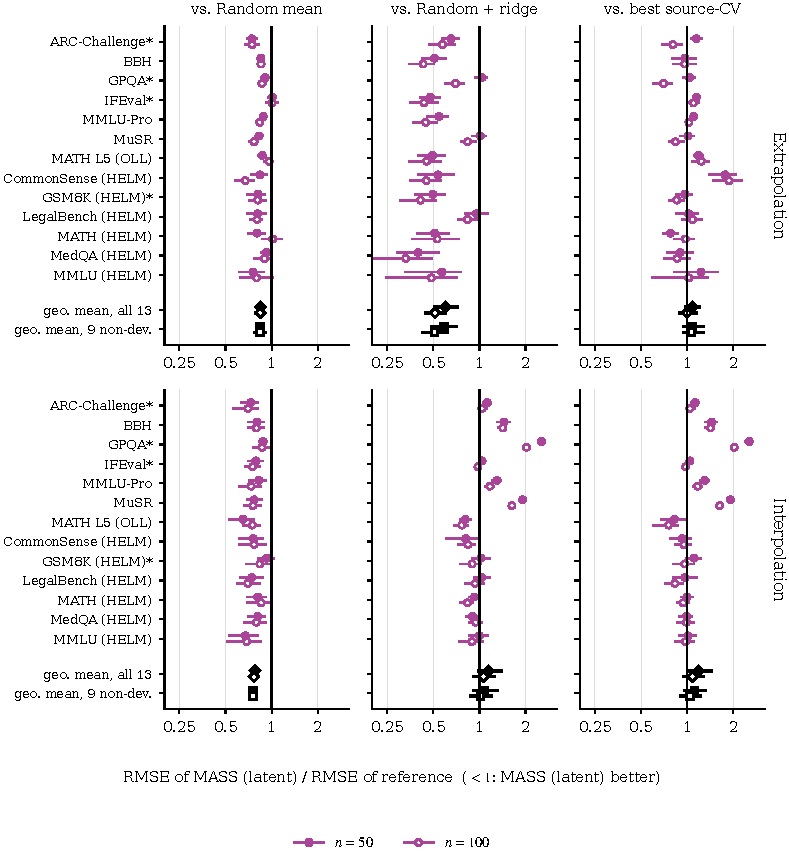
\includegraphics[width=\linewidth]{paired_rmse_mass.pdf}
\caption{As Figure~\ref{fig:paired} for the latent-only \mass{}.}\label{fig:paired-mass}\end{figure}
\begin{figure}[h]\centering
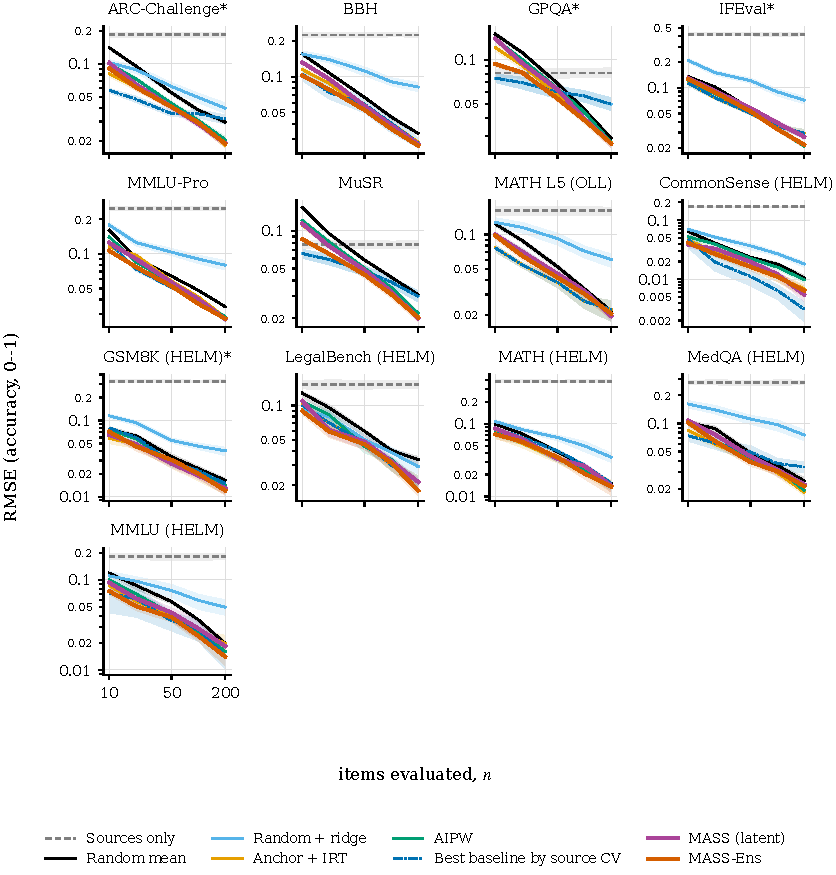
\includegraphics[width=\linewidth]{budget_grid_extrap.pdf}
\caption{Per-benchmark RMSE versus $n$, extrapolation.}\end{figure}
\begin{figure}[h]\centering
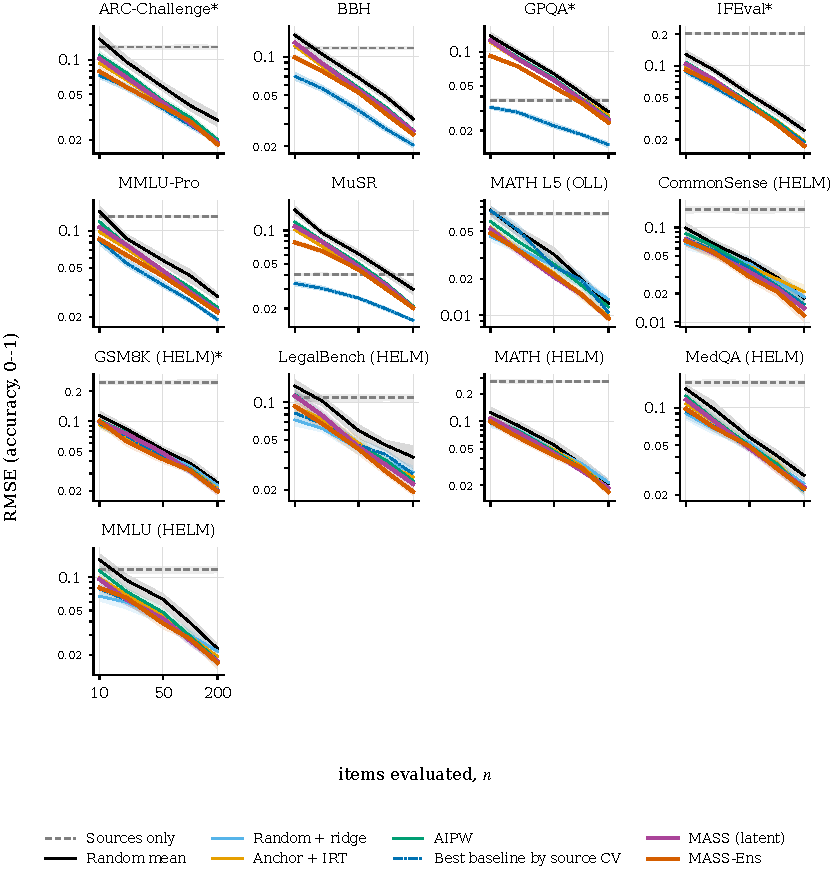
\includegraphics[width=\linewidth]{budget_grid_random.pdf}
\caption{Per-benchmark RMSE versus $n$, interpolation.}\end{figure}

\FloatBarrier
\section{Additional figures}
\begin{figure}[h]
\centering
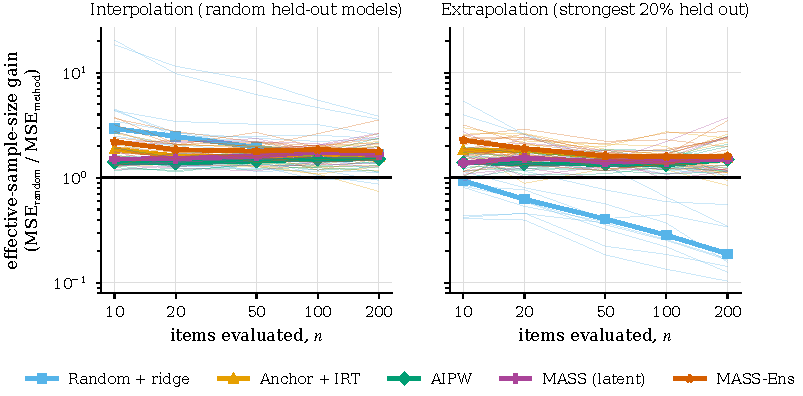
\includegraphics[width=\linewidth]{ess_gain.pdf}
\caption{Effective-sample-size gain, $(\mathrm{RMSE}_{\text{random}}/\mathrm{RMSE}_{\text{method}})^2$, per benchmark (thin) and median over benchmarks (thick). Random${}+{}$ridge falls below 1 under extrapolation.}
\label{fig:ess}
\end{figure}

\begin{figure}[h]
\centering
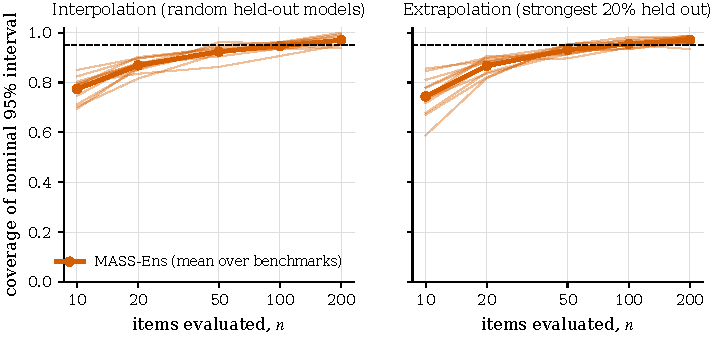
\includegraphics[width=\linewidth]{coverage.pdf}
\caption{Share of target models whose true score lies within $\pm1.96$ reported standard errors of \mass{}-Ens; thin lines are benchmarks, thick line the mean over benchmarks; dashed = nominal 95\%.}
\label{fig:cov}
\end{figure}

\begin{figure}[h]
\centering
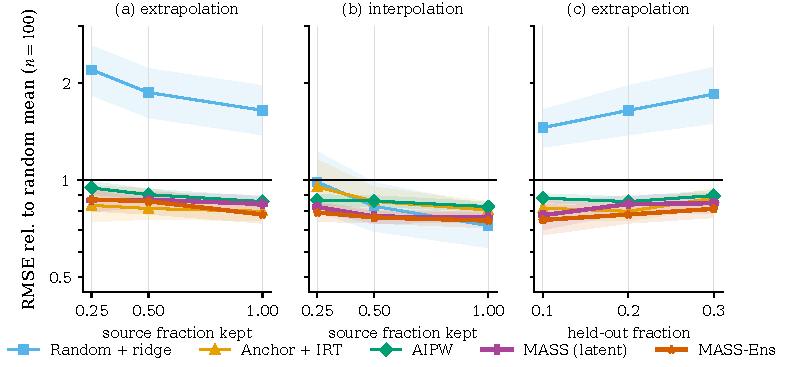
\includegraphics[width=\linewidth]{sensitivity.pdf}
\caption{RMSE ratio to the random mean ($n=100$) versus the fraction of source models kept (a, b) and the held-out fraction of strongest models under extrapolation (c).}
\label{fig:sens}
\end{figure}

\FloatBarrier
\section{Reproducibility}\label{app:repro}
Environment, data version (commit \texttt{55faff49}), seeds, commands, expected run times and the map from each table and figure to its generating script are in \texttt{README.md} and \texttt{code/README.md} of the supplementary code. The paper contains no number that is not produced by those scripts from \texttt{results/}. Statements in the text that quote a number (ratios, coverage, bias, effective-sample-size gains) are read from \texttt{results/cells.csv}, \texttt{aggregate.csv}, \texttt{coverage.csv}, \texttt{ess\_gain.csv} and \texttt{paired.csv}.
Contact with the forbidden-content rule of the task is recorded in the reproduction notes.
